%%%%%%%%%%%%%%%%%%%%%%%%%%%%%%%%%%%%%%%%%%%%%%%%%%%%%%%%%%%%%%%%%%%%%%%%%%%%%%%%
% Chapter 2: Conceptos
%%%%%%%%%%%%%%%%%%%%%%%%%%%%%%%%%%%%%%%%%%%%%%%%%%%%%%%%%%%%%%%%%%%%%%%%%%%%%%%%

%++++++++++++++++++++++++++++++++++++++++++++++++++++++++++++++++++++++++++++++
% \section{Odometría}
% \label{2:sec:3}

La odometría es el método que permite estimar la posición de un robot móvil en
el entorno en un momento determinado. 

Cabe recalcar, que la odometría no permite conocer la posición exacta de un
robot, ya que existen muchos factores externos, que provocan errores en la
obtención de los datos de entrada. Estos errores son acumulativos, por lo que
la veracidad de los resultados es inversamente proporcional a la distancia
recorrida de un robot.

A pesar de ello, la odometría ofrece una gran precisión a corto plazo y su
precio de implementación es realmente bajo, por lo que lo convierte en uno de
los pilares básicos para la navegación. 

Dependiendo de la tecnología utilizada para cálcular la odometría, se puede 
hablar de diferentes tipos.

%--------------------------------------
\subsection{Odometría mecánica}
% https://es.wikipedia.org/wiki/Odometr%C3%ADa
La odometría mecánica se base en el estudio del giro de las ruedas de un robot.
Conociendo el radio de las ruedas, mediante las revoluciones de las mismas es
posible determinar con sencillas ecuaciones el avance del robot.

Sin embargo esta sencilla solución tiene varios inconvenientes a tratar:

\begin{itemize}
  \item \textbf{Las ruedas:} las ruedas utilizadas deben contar con las mismas
  características, pero en muchas cosasiones el diámetro de las ruedas es
  diferente, o simplemente el diámetro no se corresponde con las
  especificaciones dadas por el fabricante. Por otro lado es necesario que las
  ruedas se encuentren bien alineadas.
  \item \textbf{El entorno:} la superficie por donde se mueve el robot puede no
  ser la adecuada. Dependiendo de la composición del suelo (gravilla, hierba,
  baldosas, etc), el robot puede resbalar, derrapar o incluso encontrarse sin
  ingún punto de contacto con el suelo. Por otra parte, una superficie
  desnivelada o llena de obstáculos inesperados también supone un problema para
  obtener la odometría.
\end{itemize}


%--------------------------------------
\subsection{Odometría visual}
% https://prezi.com/tl9fmj3cs4ai/sistema-de-odometria-visual-estimacion-de-la-localizacion-d/
La odometría visual permite estimar el movimiento y la posición de un robot
móvil a partir de las imágenes capturadas por una o más cámaras en el propio
sistema. De forma sencilla, si se comparan las imágenes obtenidas en un instante
t1 respecto a otras imágenes obtenidas en un instante t2, se puede calcular la
diferencia existente en un punto determinado de la imagen. Si dicho punto está
más cerca, quiere decir que el robot ha avanzado.

Pero a partir de las imágenes ¿cómo se puede determinar la distancia de un
objeto respecto al robot? En función del tamaño del objeto en la escena. Si en
la nueva escena las dimensiones espaciales de un objeto son mayores que la
anterior escena, quiere decir que se ha avanzado, y viceversa. En un sistema
esterereoscópico se comparan la diferencia respecto al eje x (disparidad) entre
la imagen izquierda y derecha. La distancia de un objeto es inversamente
proporcional a la disparidad presente, es decir, si un objeto presenta una gran
disparidad en la escena significa que se encuentra cerca. Cuanto más lejano esté
el objeto la disparidad será menor.

% \begin{wrapfigure}{l}{0.5\textwidth}
%   \vspace{-20pt}
%   \begin{center}
%     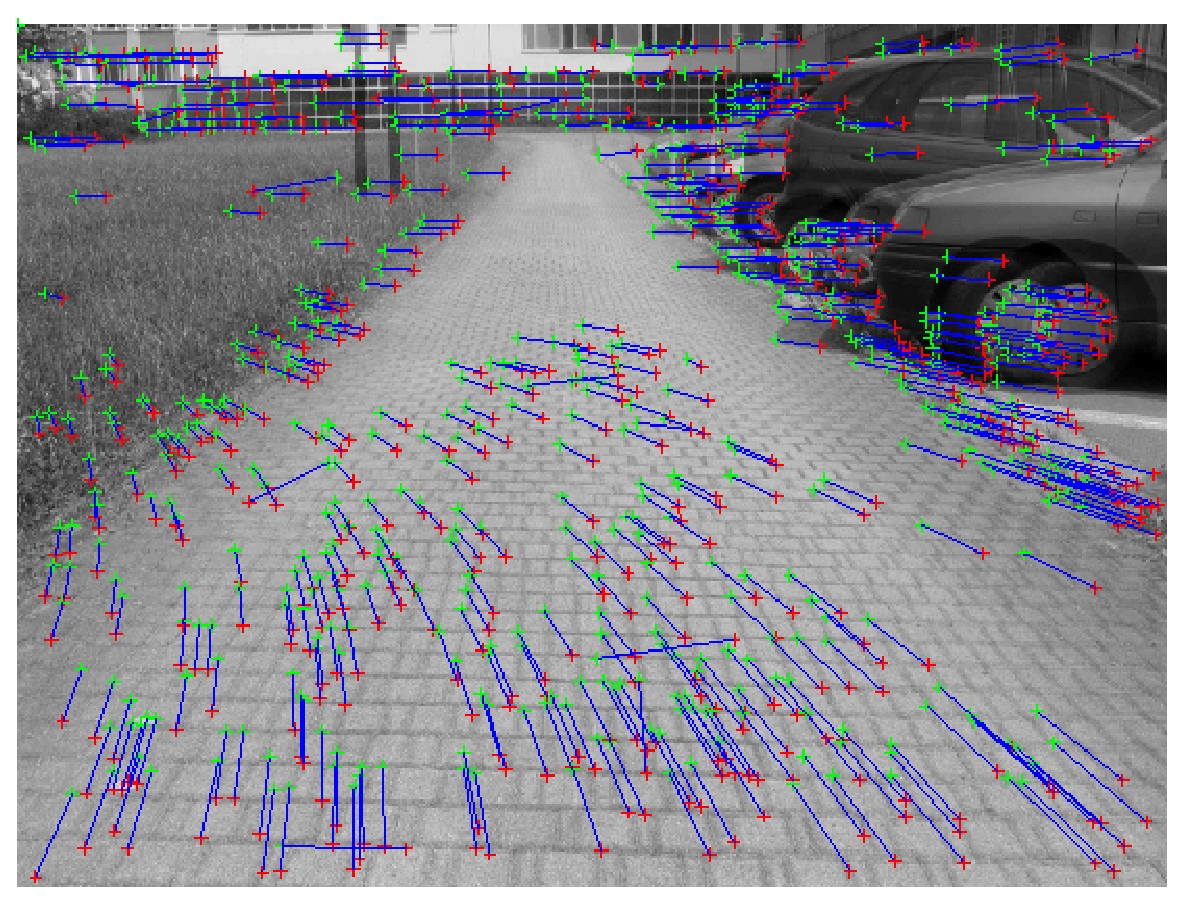
\includegraphics[width=0.48\textwidth]{images/cap2/OdometriaVisual.eps}
%   \end{center}
%   \vspace{-20pt}
%   \caption{Disparidad en odometría visual}
%   \vspace{-10pt}
%   \label{fig:OdometriaVisual}
% \end{wrapfigure}

\begin{minipage}{\linewidth}
    \centering
    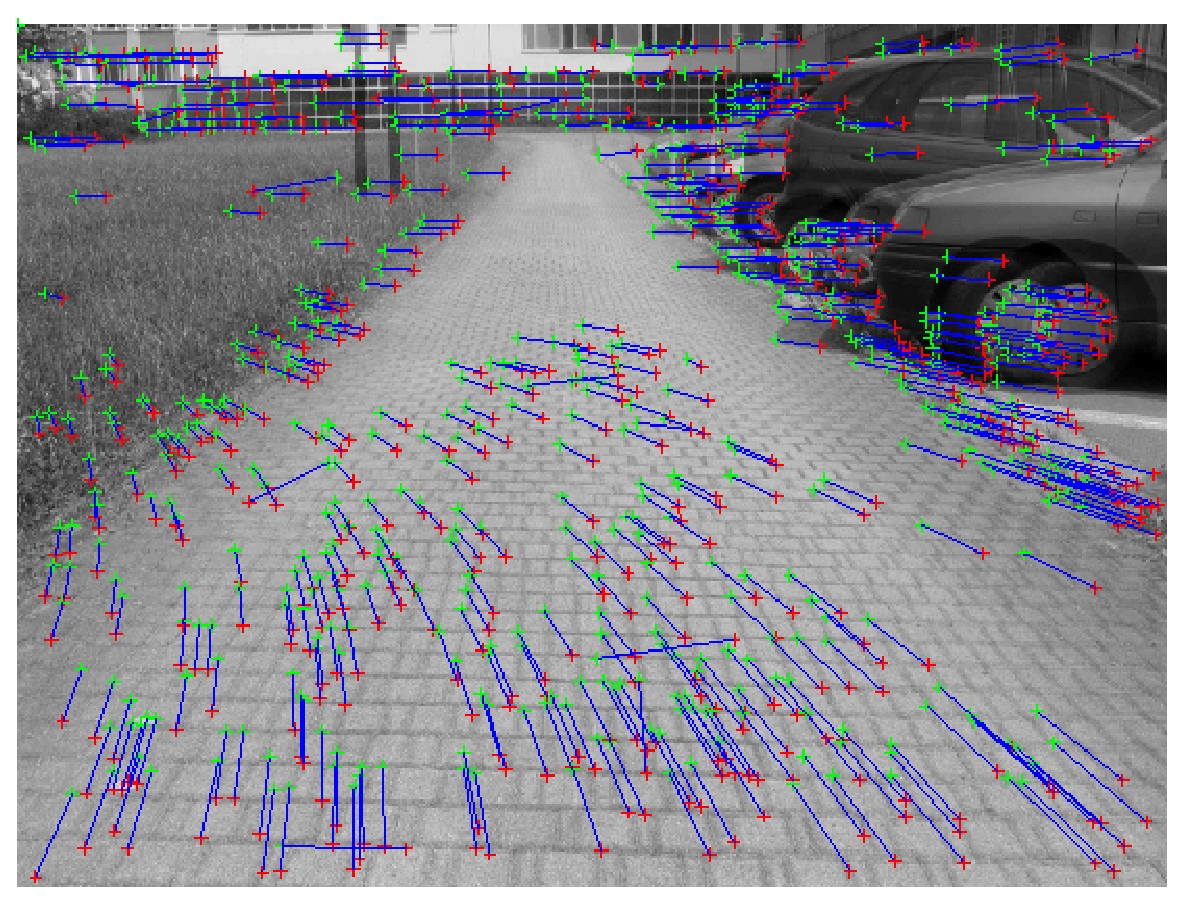
\includegraphics[width=0.5\textwidth]{images/cap2/OdometriaVisual.eps}
    \captionof{figure}{Disparidad en odometría visual}
    \label{fig:OdometriaVisual}
\end{minipage}

La odometría visual es la alternativa utilizada en robots móviles que no cuentan
con ruedas: androides, robots voladores, etc. Aunque también es bastante
frecuente encontrar la odometría visual junto con la odométría mecánica como
apoyo.

La odometría visual cuenta con los siguientes inconvenientes a tener en cuenta:

\begin{itemize}
  \item \textbf{Las cámaras:} para funcionar correctamente, es necesario que las
  cámaras estén calibradas. Por otra parte, si se utiliza un sistema
  estereóscopico se necesita verificar que la distancia entre las cámaras sea la
  correcta.
  \item \textbf{El entorno:} las cámaras son muy sencibles a los cambios bruscos
  de las condiciones del entorno como la luminosidad. También hay que tener en
  cuenta que las escenas son dinámicas, por lo que muchos objetos aparecen y
  desparecen dela escena o se mueven con mucha frecuencia en la escena, y esto
  puede suponer un importante problema.
\end{itemize}
    
Tanto la odometría mecánica como la visual presentan varios problemas para
estimar la posición y orientación del robot, sin embargo, combinando ambas se
pueden conseguir resultados más consistentes. Por ejemplo: en aquellos casos
donde la odometría mecánica no coincide con los datos visuales debido a una
superficie inconsistente, se confía en la odometría visual. Por otra parte,
cuando las condiciones lumínicas no son adecuadas, se confía en la odometría
mecánica.

%++++++++++++++++++++++++++++++++++++++++++++++++++++++++++++++++++++++++++++++
